\chapter{Pruebas de escala}
Con el entorno de simulación construido, el siguiente objetivo es realizar pruebas de escala sobre la arquitectura. Este trabajo consiste de dos etapas. La primera sección explica la primera de ellas, que es verificar cómo funciona la arquitectura para topologias de escala. Habiendo completado esta etapa, se pasa a realizar estudios de escala sobre la cantidad de servicios. En este capítulo se explicará el propósito de cada prueba, las condiciones bajo las cuales se ejecuta cada una de ellas (topologias, tipos de tráfico, etc) y por último, los resultados que arrojan. Todas las pruebas fueron realizadas en una máquina virtual con 3590 MB de RAM, procesador Intel Core i5-5200u a 2,2 GHz y Lubuntu 14.04 como sistema operativo.

Como se explicará mas adelante en el capítulo, en estas pruebas se utilizarán ciertas topologias creadas manualmente. Más allá de los detalles de cada topología, los siguientes puntos serán comunes a todas ellas.
\begin{itemize}
	\item Habrá un conjunto de RAUSwitch, conectados de acuerdo a lo que dicte cada topología.
	\item Existirán dos subredes cliente. Serán implementadas por un QuaggaRouter y un RAUHost cada una (recordar las clases del entorno virtual). Los RAUHost serán los remitentes y destinatarios del tráfico que pasará por la red. Esos datos se generarán con el comando \textit{ping} y la herramienta \textit{iperf}. Estas dos subredes tendrán una ubicación variable en cada topología, ya que se probará con distintos caminos entre ellas. Por esta razón, se omiten en las futuras imágenes de las topologias.
	\item El controlador se conectará con un switch virtual genérico (gracias a la clase Switch de Mininet, en el modo \textit{standalone}), que a su vez se conectará con los RAUSwitch. Esta será la red de gestión. Por simplicidad, dicha red se omitirá en las futuras imágenes.
\end{itemize}

\section{Topologias de escala}
Es importante poder asegurar que la arquitectura puede ser fácilmente migrada a redes reales. Para poder asegurar esto, es necesario comprobar que topologias con grandes cantidades de nodos no generan problemas inesperados. También se busca determinar el impacto de topologias grandes y complejas en el tiempo de cálculo y configuración de una VPN. Dado que en el proyecto RRAP se contaba con cuatro dispositivos, este tipo de pruebas no han sido realizadas hasta el momento.

\subsection{Descripción del escenario}
La idea principal de este escenario consiste simplemente en levantar cierta topología, dar de alta una VPN entre las dos subredes cliente y analizar el comportamiento que esto genera. Los puntos específicos que se estudiarán se detallan a continuación: \\ \\
\textbf{Algoritmo de ruteo} \\
 Se verifican dos aspectos claves: que el camino se corresponde con el camino esperado (calculado previamente de forma manual), y que el camino es correctamente instalado en forma de reglas de reenvío (en base a conmutación de etiquetas MPLS) en las respectivas tablas de flujos OpenFlow de cada nodo del camino. Todo esto se puede comprobar analizando las tablas de flujos de cada nodo, que se pueden ver utilizando el comando \textbf{dump-flows} de Open vSwitch. También se puede utilizar la interfaz gráfica de RAUFlow. Desde las tablas de flujos se puede reconstruir el camino que computó la aplicación, y también comprobar que los flujos manipulan correctamente las etiquetas MPLS. \\ \\
\textbf{Clasificación de tráfico} \\
La idea es verificar que realmente se están asignando las etiquetas MPLS al tráfico entrante, así como comprobar que el mismo es reenviado por los nodos correctos. Para probar esto se utilizará una VPN de capa 3, que permitirá tráfico con ethertype 0x0800, es decir, del protocolo IPv4. Se generará tráfico de este tipo utilizando el comando \textbf{ping} y la herramienta \textbf{iperf}. Con la herramienta tcpdump, se verificará que el tráfico pasa correctamente por cada nodo del camino. \\ \\
\textbf{Tiempo de creación de una VPN} \\
El objetivo aquí es estudiar como impacta el tamaño de la topología y el largo del camino en el tiempo que demora la arquitectura en establecer una VPN. Se espera que ese tiempo sea influenciado en gran medida por dos factores: el tiempo que demora en calcular el camino óptimo y el tiempo que demora en configurar los flujos en cada nodo. Con ayuda de un script en Python, se mandarán pedidos POST al controlador para dar de alta los servicios, y se registrará el tiempo de respuesta con ayuda de los logs del controlador. \\ \\
Las topologias que se usarán son las siguientes:
\begin{itemize}
	\item \textbf{Básica}: 4 nodos en topología de full mesh. Es la utilizada en el prototipo físico.
	\item \textbf{Chica}: topología arbitraria de 11 nodos (fuente: Topology Zoo). Figura \ref{fig:topo_chica}.
	\item \textbf{Mediana}: topología arbitraria de 45 nodos (fuente: Topology Zoo). Figura \ref{fig:topo_mediana}.
	\item \textbf{Grande}: topología de tipo arborescente compuesta por 105 nodos.
\end{itemize}

\begin{figure}[t]
\caption{Topología chica}
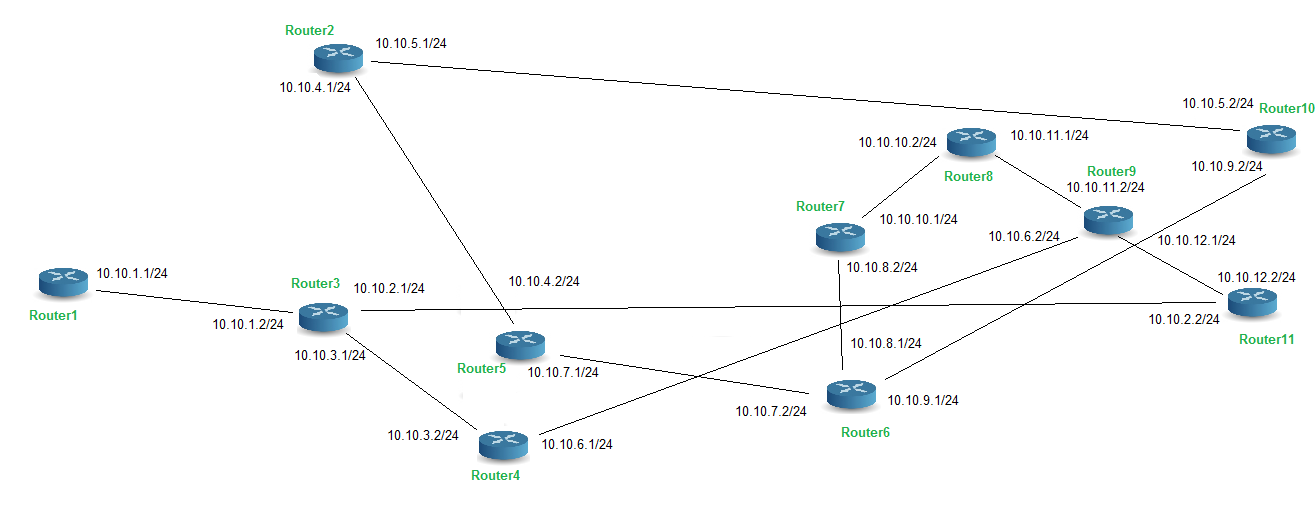
\includegraphics[scale=0.4]{Pruebas/topo_chica}
\centering
\label{fig:topo_chica}
\end{figure}

\begin{figure}[t]
\caption{Topología mediana}
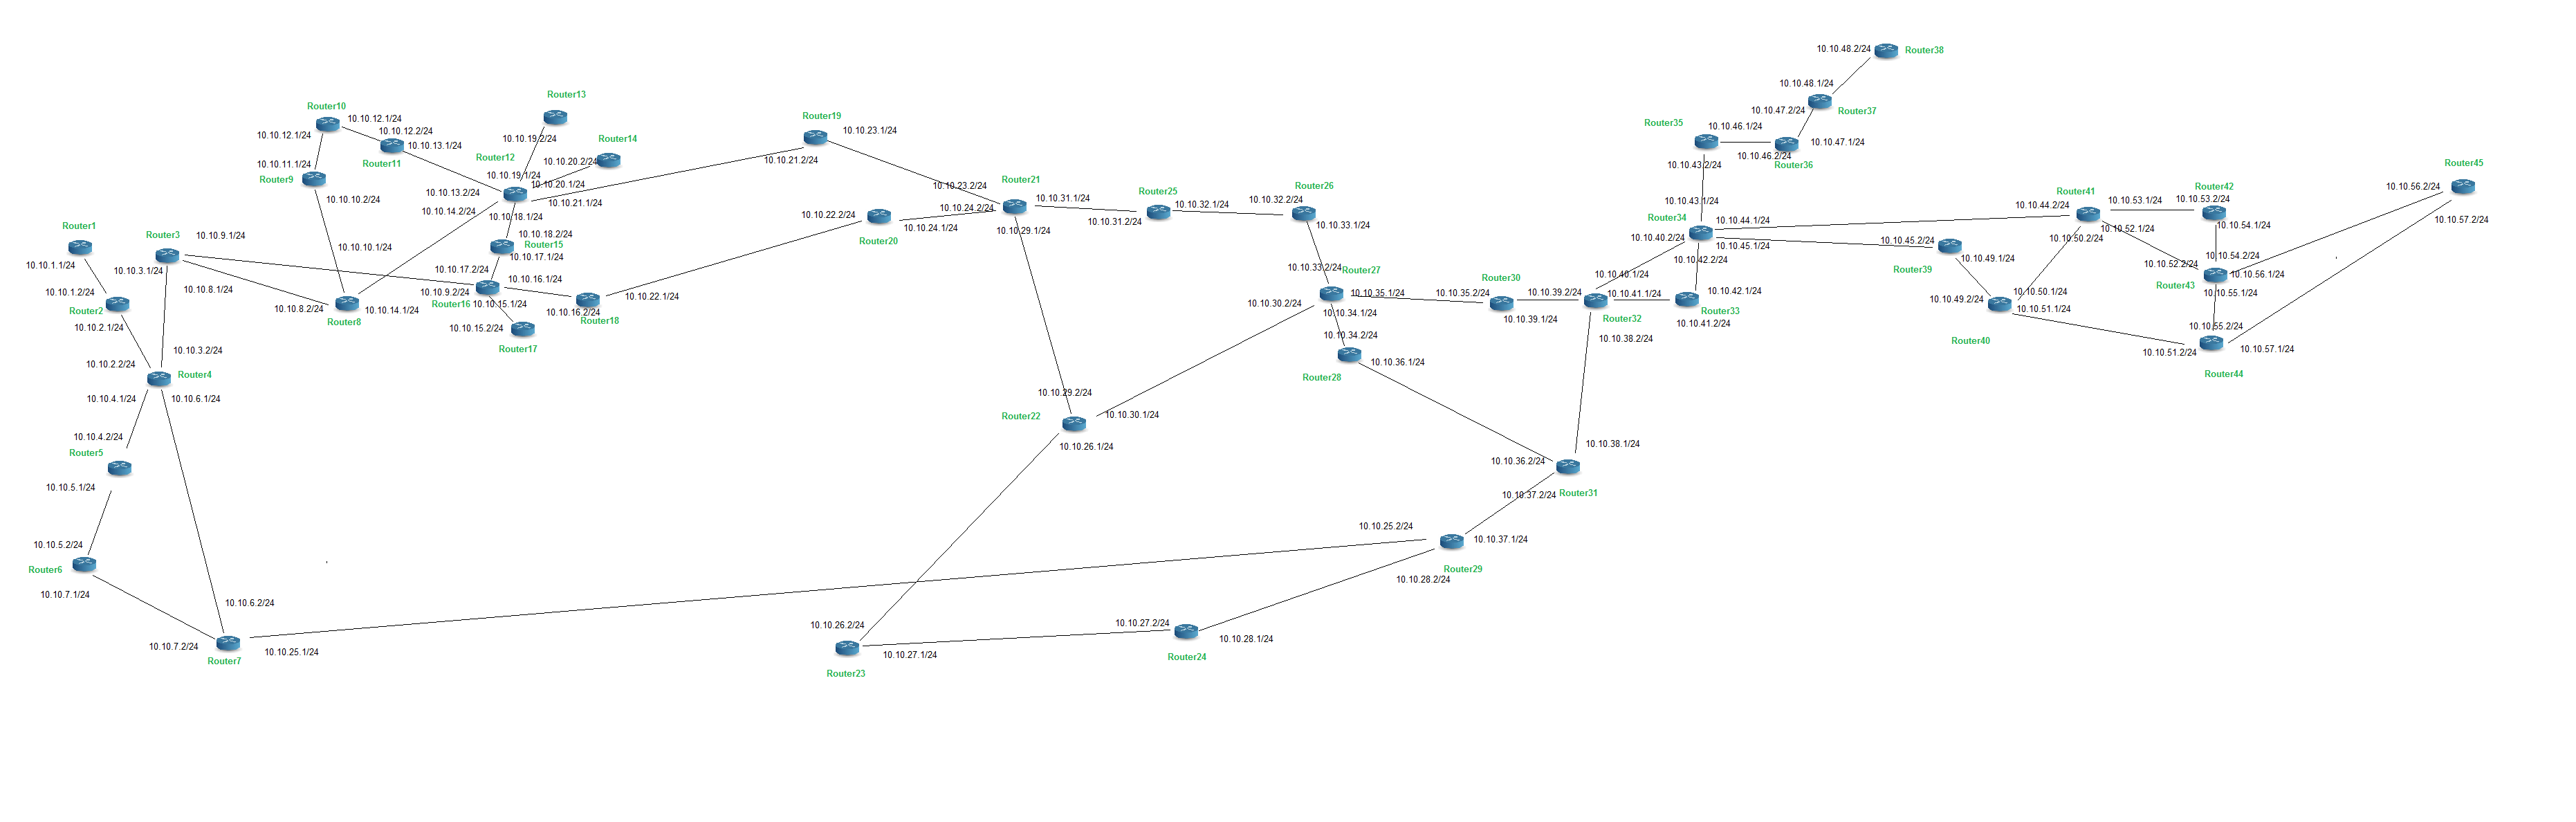
\includegraphics[scale=0.15]{Pruebas/topo_mediana}
\centering
\label{fig:topo_mediana}
\end{figure}

\subsection{Resultados y observaciones}
Esta prueba se separa en dos etapas. La primera se concentra en los dos primeros focos de estudio que se listaron en la descripción del escenario. Esto quiere decir que en la primera etapa se busca verificar que la arquitectura maneja sin problemas las topologias de estudio. En la tabla \ref{table:problemas_por_topologia} se detallan los comportamientos observados para algunos de los casos estudiados. En ella se indica con una X los aspectos que funcionaron correctamente para cada caso. Los aspectos que se estudian son: se crea con éxito el servicio, el camino que se calcula es correcto, los flujos de cada nodo del camino son correctos, y se clasifica correctamente el tráfico. Si se cumplen todos ellos, quiere decir que la VPN se crea correctamente y el tráfico pasa sin problemas por la misma.

\begin{table}[ht]
\caption{Resultados por topología.}
% title of Table
\centering 
% used for centering table
\begin{tabular}{c c c c c}
\hline\hline
Largo del camino (topología) & Servicio & Camino & Flujos  & Clasificación de tráfico \\ [0.5ex]
\hline
1 (básica) & X & X & X & X \\
7 (chica) & X & X &  &  \\
10 (mediana) &  &  &  &  \\
14 (grande) &  &  &  &  \\ [1ex]
\hline
\end{tabular}
\label{table:problemas_por_topologia}
\end{table}
Se pueden observar como mínimo dos problemas. El primero es que en el caso de la topología chica y un camino de 7 saltos, los flujos están en los nodos correctos (los del camino más corto entre las subredes cliente) ,pero los mismos no son correctos. EXPLICACIÓN.

El segundo problema detectado es que para el caso del camino de 10 saltos en la topología mediana, y el de 14 saltos en la topología grande, el servicio ni siquiera llega a crearse correctamente, es decir, la aplicación sufre una excepción de Python al intentar hacerlo. EXPLICACIÓN.

***Mencionar el nuevo error que causa error 500 al crear servicios en la topología mediana con camino de largo 13.*** \\

Con los errores de código solucionados y habiendo asegurado que las VPN se pueden crear y usar sin problemas para todas las topologias, se pasa a la segunda etapa de esta prueba, que consiste en estudiar el impacto del largo del camino y la cantidad de nodos en el tiempo de creación de una VPN. Las tablas \ref{table:tiempo_vpn_2} y \ref{table:tiempo_vpn_3} muestran para cada topología, los distintos largos de camino probados y su respectivo tiempo. La tabla \ref{table:tiempo_vpn_2} muestra los resultados cuando se trata de una VPN de capa 2, y la tabla \ref{table:tiempo_vpn_3} lo hace cuando es VPN de capa 3. Las celdas con \textit{N/C} indican que no es posible crear un camino de ese largo para esa topología.

\begin{table}[ht]
	\caption{Tiempo de demora en crear una VPN de capa 2. El tiempo se mide en m/s.}
	\centering 
	\begin{tabular}{c c c c c}
		\hline\hline
		Largo del camino & Básica & Chica & Mediana  & Grande \\ [0.5ex]
		\hline
		1 & 58.3 & 65.0 &  &  \\
		2 & N/C & 100.8 &  &  \\
		4 & N/C & 105.2 &  &  \\
		6 & N/C & 107.8 &  &  \\
		8 & N/C & 109.6 &  &  \\
		10 & N/C & N/C &  &  \\
		12 & N/C & N/C &  &  \\
		14 & N/C & N/C &  &  \\ [1ex]
		\hline
	\end{tabular}
	\label{table:tiempo_vpn_2}
\end{table}

\begin{table}[ht]
	\caption{Tiempo de demora en crear una VPN de capa 3. El tiempo se mide en m/s.}
	\centering 
	\begin{tabular}{c c c c c}
		\hline\hline
		Largo del camino & Básica & Chica & Mediana  & Grande \\ [0.5ex]
		\hline
		1 & 6.3 & 6.8 &  &  \\
		2 & N/C & 7.8 &  &  \\
		4 & N/C & 9.4 &  &  \\
		6 & N/C & 15.1 &  &  \\
		8 & N/C & 12.0 &  &  \\
		10 & N/C & N/C &  &  \\
		12 & N/C & N/C &  &  \\
		14 & N/C & N/C &  &  \\ [1ex]
		\hline
	\end{tabular}
	\label{table:tiempo_vpn_3}
\end{table}
*** Algunas conclusiones de las pruebas  de tiempo

*** Algunas conclusiones generales

EXPLICAR PROBLEMA DEL MTU CON IPERF: Hay que reducir 5 o 10 bytes (dependiendo de si el servicio usa 1 o 2 niveles de etiquetas MPLS) al MTU para que el tráfico pase.\\

\section{Escala de servicios y flujos}
Entre los requerimientos de la RAU2 se encuentra el de la escalabilidad de usuarios. En particular, se espera alcanzar en un mediano plazo un total de 11.000 docentes, 7.000 funcionarios y 140.000 estudiantes (de acuerdo a los requerimientos relevados por el proyecto RRAP). Esto implica que la red será sujeta a importantes cantidades de servicios y flujos distintos. He aquí la relevancia de las pruebas en la presente sección. Mediante el entorno virtual, se someterá la arquitectura a una cantidad de servicios relativamente grande y de esta forma se podrían identificar posibles puntos de falla, o umbrales bajo los cuales debe mantenerse la red para funcionar con buen rendimiento. Dado que en esta prueba también se utilizarán topologias grandes, hay que recordar la misma es posible gracias a la corrección de los errores que se explicó en la sección anterior. También es importante recordar que aunque el entorno de simulación permite hacer un valioso estudio de escalabilidad, no generará resultados en lo que refiere a la performance de la arquitectura. Recordar sección 3.3.2, donde se explica que cada instancia de Open vSwitch se ejecuta en modo user-space, y por ende procesa los paquetes de forma bastante lenta.

\subsection{Descripción del escenario}
La idea principal del escenario es crear muchas VPN y analizar los comportamientos que esto genera. Se utiliza una VPN punto a punto de capa 3 para conectar dos subredes cliente, y se utiliza \textit{iperf} para generar tráfico TCP y medir el ancho de banda entre los dos RAUHost. Para cargar a la arquitectura con servicios, se crean múltiples VPN de capa 2 entre las subredes, variando los valores de los cabezales VLAN\_ID y VLAN\_PCP (pudiendo crear un total de 32.768 combinaciones distintas) para que toda VPN sea distinta de las demás. De esta forma, existirán múltiples VPN pero solo una (la de capa 3) será utilizada. \\
Dado que cargar todas las VPN a mano en la interfaz web llevaría demasiado tiempo, se creó un servicio web que recibe como parámetro la cantidad de VPN que se desean. Cuando se hace un pedido GET a ese servicio web, se inicia el proceso de creación de las mismas. Este proceso puede tomar entre algunos minutos y varias horas, dependiendo de la cantidad. \\ \\
El objetivo es verificar los siguientes dos aspectos claves: \\ \\
\textbf{Escalabilidad interna del RAUSwitch} \\
Se estudian posibles limitaciones internas que puedan tener los dispositivos, cuando deben manejar grandes cantidades de flujos. Es posible que a medida que crece su tabla de flujos, demoren más en encontrar el flujo que se corresponde con cada paquete que reciben. Si pasa esto, el ancho de banda debería ser afectado negativamente por la cantidad de flujos en sus tablas. El ancho de banda se medirá con la herramienta \textit{iperf}.  \\ \\
\textbf{Escalabilidad en servicios} \\
Se estudian posibles problemas que puedan tener la arquitectura de la red o la aplicación del controlador para manejar grandes cantidades de servicios e información. \\ \\
Esta prueba se repite para las mismas topologias que la prueba anterior, es decir: básica (4 nodos), chica (11 nodos), mediana (45 nodos) y grande (105 nodos).

\subsection{Resultados y observaciones}

En lo que respecta a los anchos de banda medidos, los resultados de la prueba con cada topología se pueden ver en la tabla \ref{table:escala_de_servicios}. Se pueden observar dos hechos interesantes. El primer resultado que se puede estudiar, es que el ancho de banda es más bajo a medida que se incrementa la cantidad de nodos y/o el largo del camino. Esto se explica desde dos ángulos. El primero es que al tener que pasar por un camino más largo, un paquete debe ser inspeccionado y reenviado más veces. Por lo tanto, este resultado debería sería visible también en un ambiente de prueba con dispositivos físicos. El segundo ángulo que explica este resultado radica en el entorno virtual mismo. Al tener que manejar más nodos virtuales, el sistema operativo anfitrión tiene menos recursos para dedicar a cada uno. Esto quiere decir que tanto las instancias de \textit{iperf} que se encargan de recibir y enviar los paquetes, como las instancias de Open vSwitch que los procesan en cada nodo del camino, tendrán menos tiempo de CPU para realizar su tarea. \\

\begin{table}[ht]
	\caption{Anchos de banda, en Kbits/s, medidos para cada caso.}
	\centering 
	\begin{tabular}{c c c c c}
		\hline\hline
		\# de VPN & Básica & Chica & Mediana  & Grande \\ [0.5ex]
		\hline
		1 & 893 & Y & W & Z \\
		3000 & 887 & Y & W & Z  \\
		6000 & 887 & Y & W & Z \\
		9000 & 890 & Y & W & Z \\
		12000 & 885 & Y & W & Z \\
		15000 & 886 & Y & W & Z \\ [1ex]
		\hline
	\end{tabular}
	\label{table:escala_de_servicios}
\end{table}

El otro resultado que se puede observar en la tabla \ref{table:escala_de_servicios}, es que el ancho de banda es constante para un camino y topología, sin importar la cantidad de VPN existentes en el momento. Como se explica en el primer objetivo de esta prueba, se busca determinar si la existencia de muchos flujos en la tabla, implica que el switch OpenFlow demora más tiempo en encontrar el flujo que corresponde para un paquete entrante, y por lo tanto el mismo demora más en ser forwardeado. Si esto fuera así, debería haber un impacto directo en el throughput. El máximo de VPN con el que se probó fueron 15.000. Cada VPN de capa 2 está compuesta por dos servicios de capa 2, y cada uno de esos servicios introduce 42 flujos en cada nodo del camino. Esto quiere decir que cada uno contiene alrededor de 1.260.000 flujos en su tabla. \\
La explicación de porqué esa cantidad de flujos no afecta el ancho de banda se encuentra en la especificación de la herramienta Open vSwitch, que utiliza la arquitectura y el entorno virtual para implementar OpenFlow. Dicha herramienta realiza cacheo de flujos. Eso quiere decir que cuando un paquete de datos de un determinado flujo llega por primera vez a un nodo, este paquete es enviado al pipeline de OpenFlow para determinar qué acción se debe tomar. Luego de realizada, esta acción es escrita en la caché, y tiene un tiempo de vida de entre 5 y 10 segundos. Si en ese período de tiempo llega otro paquete del mismo flujo, no hay necesidad de enviar el paquete al pipeline, porque ya se sabe cuales son las acciones a tomar para ese paquete. Por lo tanto, si un flujo de datos es constante y rápido, el tamaño de la tabla de OpenFlow no afectará el tiempo de decisión, ya que sólo el primer paquete de ese flujo deberá pasar por el pipeline. \\
Mediante el comando 'ovs-appctl dpctl/show' de Open vSwitch, podemos examinar las estadísticas de la cache del datapath. Con el parámetro opcional \textit{target} se apunta el comando a cada instancia de Open vSwitch, y por ende, a cada nodo. En las figuras \ref{fig:iperf_sample} y \ref{fig:cache_sample} se observa, por un lado, la salida de 'iperf' luego de hacer tres ejecuciones, y por otro, las estadísticas del nodo 'alice' luego de dichas ejecuciones. En la sección 'lookups' se detallan cuantos 'hits' y 'miss' de caché han ocurrido hasta el momento, y 'flows' indica cuantos flujos activos hay en el momento en la caché. \\ \\
Otro objetivo de la prueba es determinar si la arquitectura, y en particular la aplicación, tienen algún problema para manejar muchos servicios. No se detectó ninguna problema de esa índole. Sin ser una limitación, pero sí un factor importante, hay que recordar que los datos que maneja el controlador (entre ellos, los servicios) están en memoria. Por lo tanto se podrá agregar servicios mientras la computadora subyacente tenga suficiente memoria. La creación de 15.000 VPN (30.000 servicios) aumenta el consumo de memoria del controlador en 412 Mb, por lo que un servicio ocupa alrededor de 14 Kb. A modo de ejemplo, si extrapolamos ese número a una computadora que puede dedicar 4 Gb de RAM al controlador, llegamos a que dicho controlador podrá mantener alrededor de 300.000 servicios. \\

También se observó un comportamiento que no se esperaba. Se detectó que a medida que hay más VPN creadas, la red demora más tiempo en crear una nueva VPN. La siguiente gráfica ilustra este comportamiento. \\ \\
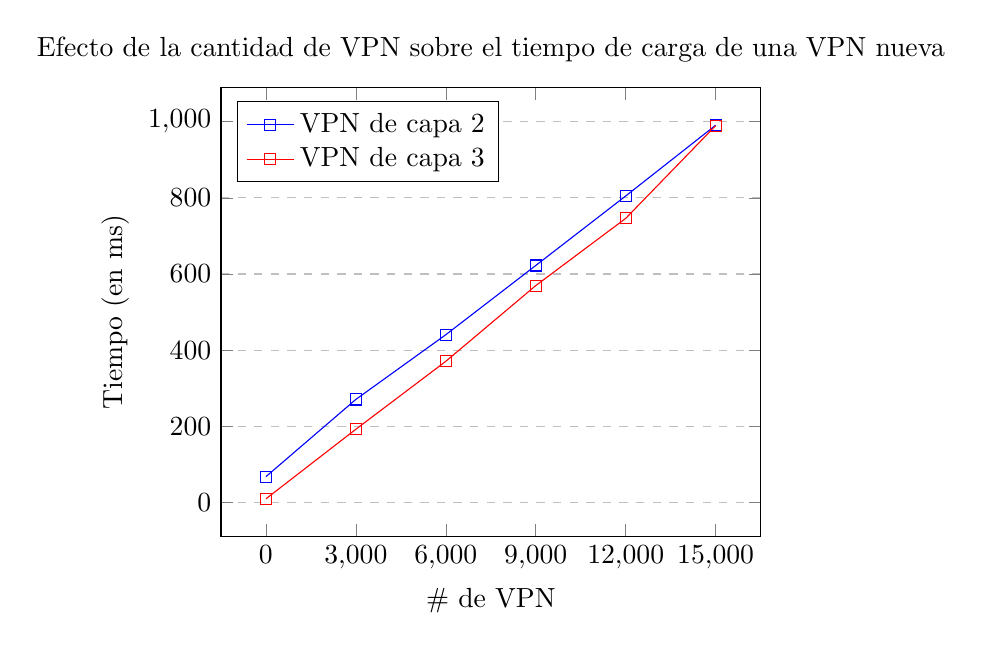
\begin{tikzpicture}
\begin{axis}[
	title={Efecto de la cantidad de VPN sobre el tiempo de carga de una VPN nueva},
	xlabel={\# de VPN},
	ylabel={Tiempo (en ms)},
	xtick={0,3000,6000,9000,12000,15000},
	ytick={0,200,400,600,800,1000,1200},
	scaled x ticks = false,
	x tick label style={/pgf/number format/fixed},
	legend pos=north west,
	ymajorgrids=true,
	grid style=dashed,
]
\addplot[
	color=blue,
	mark=square,
	]
	coordinates {
		(1,68.2)(3000,270.9)(6000,440.7)(9000,622.4)(12000,804.8)(15000,990.5)
	};
	\addlegendentry{VPN de capa 2}
\addplot[
	color=red,
	mark=square,
	]
	coordinates {
		(1,10.0)(3000,192.6)(6000,370.9)(9000,569.6)(12000,746.0)(15000,989.3)
	};
	\addlegendentry{VPN de capa 3}
\end{axis}
\end{tikzpicture}
Se puede ver que el tiempo de carga aumenta de forma lineal con la cantidad de VPN existentes. Una posible explicación para esto puede ser que al tener más flujos, cada nodo demora más en insertar los flujos nuevos en su tabla. Otra posible razón puede ser que mientras más datos en memoria, más lento se comporta la aplicación RAUFlow. \\ \\

\begin{figure}[t]
	\caption{Estadísticas de cache de flujos del nodo 'alice'.}
	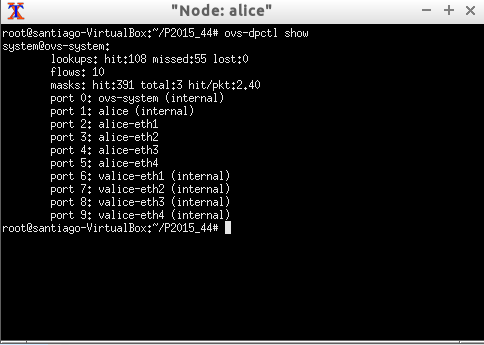
\includegraphics[scale=1]{Pruebas/cache_sample}
	\centering
	\label{fig:cache_sample}
\end{figure}

\begin{figure}[t]
	\caption{Resultado de la ejecución de 3 pruebas iperf en el host h1.}
	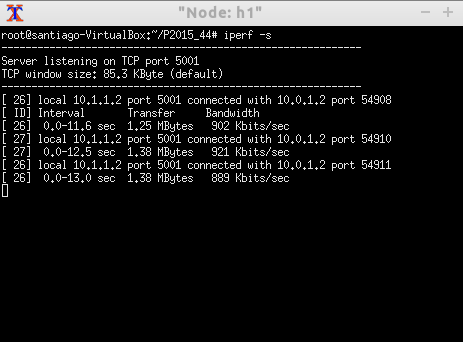
\includegraphics[scale=1]{Pruebas/iperf_sample}
	\centering
	\label{fig:iperf_sample}
\end{figure}

***Algunas conclusiones de estas pruebas.